\section{Kiến thức cơ sở}
Những kiến thức cơ sở để triển khai luận văn bao gồm kiến thức về kiểm thử phần mềm, kỹ thuật sinh ngẫu nhiên dữ liệu thử, và kỹ thuật Dynamic Symbolic Execution.

\subsection{Kiểm thử phần mềm}
\subsubsection{Các phương pháp kiểm thử}
Có nhiều phương pháp để kiểm thử phần mềm, trong đó hai phương pháp kiểm chính là kiểm thử thử tĩnh và kiểm thử động là hai phương pháp chính.

\textbf{\textit{Kiểm thử tĩnh (Static testing)}}: Là phương pháp kiểm thử phần mềm bằng cách duyệt lại các yêu cầu và các đặc tả bằng tay, thông qua việc sử dụng giấy, bút để kiểm tra tính logic từng chi tiết mà không cần chạy chương trình. Kiểu kiểm thử này thường được sử dụng bởi chuyên viên thiết kế, người viết mã lệnh chương trình. Kiểm thử tĩnh cũng có thể được tự động hóa bằng cách thực hiện kiểm tra toàn bộ hệ thống thông qua một trình thông dịch hoặc trình biên dịch, xác nhận tính hợp lệ về cú pháp của chương trình.
		
\textbf{\textit{Kiểm thử động (Dynamic testing)}}: Là phương pháp kiểm thử thông qua việc chạy chương trình để kiểm tra trạng thái tác động của chương trình, dựa trên các ca kiểm thử xác định các đối tượng kiểm thử của chương trình. Đồng thời, kiểm thử động sẽ tiến hành kiểm tra cách thức hoạt động của mã lệnh, tức là kiểm tra phản ứng từ hệ thống với các biến thay đổi theo thời gian. Trong kiểm thử động, phần mềm phải được biên dịch và chạy, và bao gồm việc nhập các giá trị đầu vào và kiểm tra giá trị đầu ra có như mong muốn hay không.	
	
\subsection{Sinh dữ liệu kiểm thử}
Sinh ngẫu nhiên dữ liệu thử là một kỹ thuật kiểm thử phần mềm Black-Box, kỹ thuật này tạo ra ngẫu nhiên các giá trị đầu vào và thực thi từng giá trị đầu vào trên chương trình được kiểm thử. Kết quả đầu ra của chương trình được so sánh với các thông số kỹ thuật của phần mềm, xác định đầu ra thử nghiệm thành công hoặc không thành công \cite{myers2011art}.  

Kỹ thuật sinh ngẫu nhiên dữ liệu thử không quan tâm đến hành vi và cấu trúc bên trong của chương trình, chỉ tập trung tìm kiếm những trường hợp chương trình không hoạt động theo đặc tả kỹ thuật của chương trình. Trong phương pháp này, dữ liệu thử nghiệm được tạo ngẫu nhiên từ các đặc tả kỹ thuật của phần mềm (tức là không liên quan tới hành vi và cấu trúc của chương trình).

\lstinputlisting[label={rt}, caption = {Hàm sinh ngẫu nhiên dữ liệu thử}]{RandomTesting.cs}
Mã lệnh \ref{rt} là một hàm sinh ngẫu nhiên dữ liệu thử, chúng ta thấy hàm $testAbs$ chỉ thực hiện việc tạo giá trị đầu vào ngẫu nhiên $int x$ theo đặc tả tham số đầu vào của chương trình $myAbs$, và kiểm tra kết quả đầu ra của chương trình $assert(result >= 0)$, không quan tâm hành vi và cấu trúc bên trong của hàm $myAbs$.

\subsubsection*{Ưu điểm, hạn chế, hướng khắc phục}
Sinh ngẫu nhiên dữ liệu thử có một số ưu điểm và nhược điểm như sau:

\textit{* Ưu điểm:}
\begin{itemize}
	\item Đơn giản, dễ dàng sinh các đầu vào ngẫu nhiên
	\item Không tốn nhiều tài nguyên bộ nhớ lúc thực thi
\end{itemize}

\textit{* Hạn chế:}
\begin{itemize}
	\item Một nhánh hành vi của chương trình được kiểm thử nhiều lần với nhiều đầu vào khác nhau
	\item Có thể một số nhánh hành vi của chương trình bị bỏ qua
	\item Khó xác định khi nào việc kiểm thử nên dừng lại
	\item Không biết dữ liệu thử có duyệt được tất cả các nhánh trong chương trình hay không
\end{itemize}

\textit{* Hướng khắc phục:}
Để xác định khi nào việc kiểm thử dừng lại, hệ thống kiểm thử ngẫu nhiên có thể kết hợp với kỹ thuật Adequacy Criterion \cite{zhu1997software}. Kỹ thuật Adequacy Criterion là một kỹ thuật yêu cầu duyệt tất cả các nhánh của chương trình, bằng việc kết hợp này cho phép việc kiểm thử chỉ dừng lại khi tất cả các câu lệnh của chương trình được thực thi ít nhất một lần.

\subsection{Kỹ thuật DSE}
Dynamic symbolic execution (DSE) là một kỹ thuật duyệt tự động tất cả các đường đi có thể của chương trình bằng cách chạy chương trình với nhiều giá trị đầu vào khác nhau để tăng độ phủ của dữ liệu thử \cite{xie2009fitness}.

Dựa trên các tham số đầu vào của chương trình, DSE sẽ tạo ra các giá trị đầu vào cụ thể và thực thi chương trình với các giá trị cụ thể này. Trong quá trình thực thi, DSE sẽ ghi nhận lại ràng buộc tại các nút, phủ định lại các ràng buộc này và sinh các giá trị đầu vào thỏa điều kiện ràng buộc tại các nút rẽ nhánh này. Với một giá trị đầu vào cụ thể, DSE sẽ thực thi chương trình và duyệt được một đường đi cụ thể, quá trình thực thi này sẽ lặp lại cho đến khi duyệt hết tất cả các đường đi của chương trình.

\begin{algorithm}
	\caption{DSE}
	\begin{algorithmic}	
		\item Set J:= $\varnothing $ \Comment{J: Tập hợp các đầu vào của chương trình phân tích}
		\item loop
		\subitem Chọn đầu vào i $\notin $ J \Comment{Dừng lại nếu không có i nào được tìm thấy}
		\subitem Xuất ra i
		\subitem Thực thi P(i); lưu lại điều kiện đường đi C(i); suy ra C'(i)
		\subitem Đặt J := J $\cup $ i			
		\item end loop
	\end{algorithmic}
\end{algorithm}

\lstinputlisting[label={vddse}, caption = {Minh họa kỹ thuật DSE}]{DSE.cs}

Trong mã lệnh \ref{vddse}, chúng ta xem xét hàm test\_me với hai tham số đầu vào là $int x$ và $int y$, và hàm này không có giá trị trả về. Cách thức làm việc của DSE trên hàm $test\_me$ như sau: 

Đầu tiên, DSE tạo hai giá trị đầu vào thử nghiệm ngẫu nhiên $x$ và $y$, giả sử $x = 22$ và $y = 7$. Ngoài ra, DSE sẽ theo dõi trạng thái các giá trị đầu vào thử nghiệm của chương trình với $x$ bằng một số $x_{0}$ và $y$ bằng một số $y_{0}$.
\begin{center}
	\begin{figure}[H]
		\begin{center}
			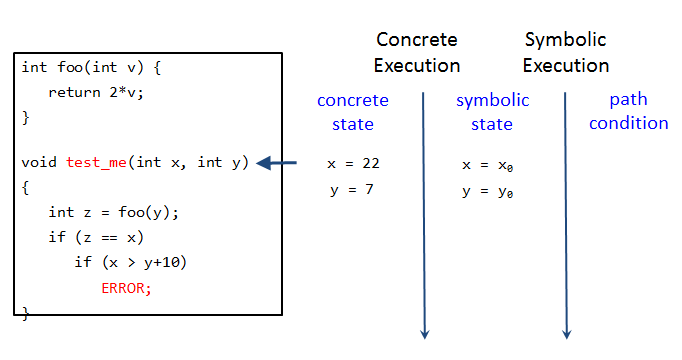
\includegraphics[scale=.4]{dse11.png}
		\end{center}
		\caption{DSE khởi tạo các giá trị đầu vào}
		\label{dse11}
	\end{figure}
\end{center}
Ở dòng đầu tiên, số nguyên $z$ được gán bằng hàm$foo(y)$. Điều này có nghĩa là $z = 14$, và ở trạng thái tượng trưng, biến $ z = 2*y_{0} $. 
\begin{center}
	\begin{figure}[H]
		\begin{center}
			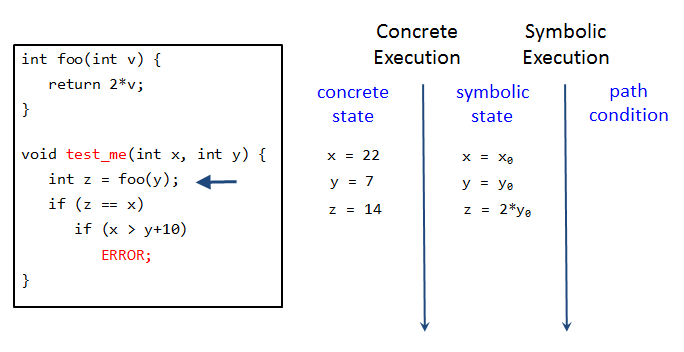
\includegraphics[scale=.4]{dse12.png}
		\end{center}
		\caption{Số nguyên Z được gán bằng hàm foo(y)}
		\label{dse12}
	\end{figure}
\end{center}

Tại nhánh $z$ == $x$, DSE nhận biết giá trị của $z$ không bằng giá trị của $x$ và lưu trữ ràng buộc này là $z != x$, và giá trị tương trưng của đường này là: $ 2*y_{0} != x_{0} $. DSE đi theo nhánh $false$ dẫn đến kết thúc chương trình.
\begin{center}
	\begin{figure}[H]
		\begin{center}
			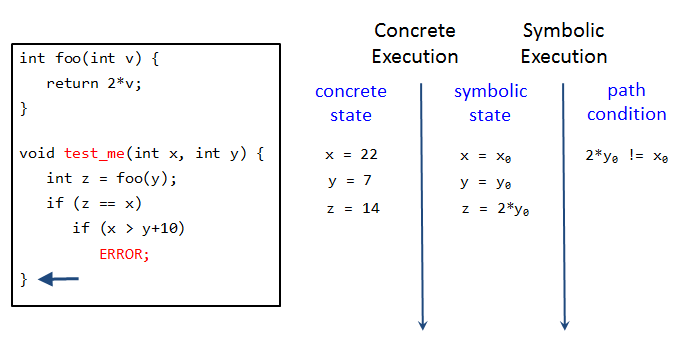
\includegraphics[scale=.4]{dse13.png}
		\end{center}
		\caption{Với điều kiện $z == x$, giá trị của  $z != x$ nên DSE chạy theo nhánh $false$  }
		\label{dse13}
	\end{figure}
\end{center}

Sau khi kết thúc chương trình, DSE sẽ quay trở lại điểm nhánh gần nhất và chọn nhánh $true$. Với mục đích này, nó phủ định ràng buộc được thêm gần nhất trong điều kiện đường dẫn $2*y_{0} != x_{0}$ thành $2*y_{0} = x_{0}$. Để thỏa mãn ràng buộc  $2*y_{0} != x_{0}$  thì hai số nguyên này sẽ là $x_{0} = 2$ và $ y_{0} = 1$.

\begin{center}
	\begin{figure}[H]
		\begin{center}
			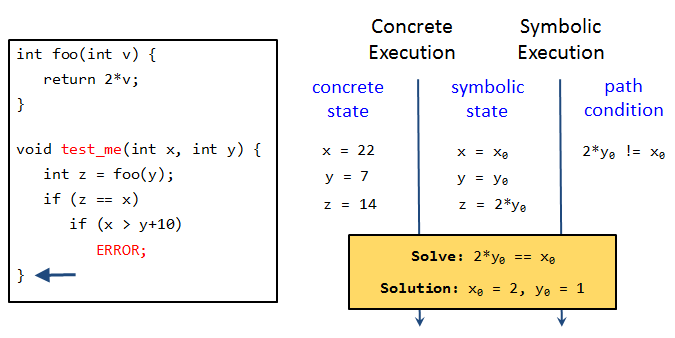
\includegraphics[scale=.4]{dse2.png}
		\end{center}
		\caption{Các giá trị DSE sinh ra sau khi thực thi chương trình lần 1}
		\label{dse2}
	\end{figure}
\end{center}

Sau đó, DSE khởi động lại hàm test\_me, lần này nó gọi các giá trị đầu vào cụ thể với giá trị: $x = 2$ và $y = 1$ được tạo ra bởi quá trình giải quyết ràng buộc trước đó. DSE tiếp tục theo dõi trạng thái các biến với $x = x_{0}$ và $y = y_{0}$.

\begin{center}
	\begin{figure}[H]
		\begin{center}
			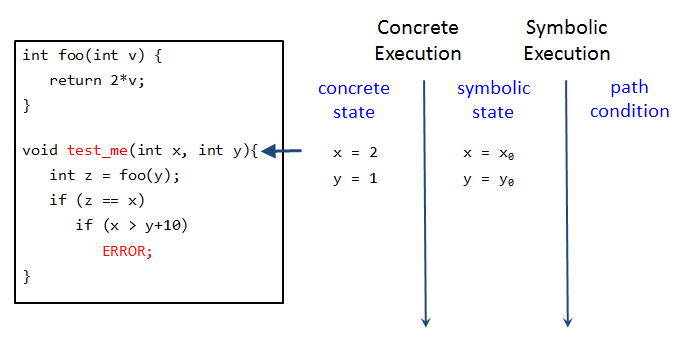
\includegraphics[scale=.4]{dse21.png}
		\end{center}
		\caption{DSE khởi động lại hàm test\_me}
		\label{dse21}
	\end{figure}
\end{center}

Sau khi thực hiện dòng đầu tiên, $z$ có giá trị cụ thể $2$ và giá trị biểu tượng $2*y_{0}$.

\begin{center}
	\begin{figure}[H]
		\begin{center}
			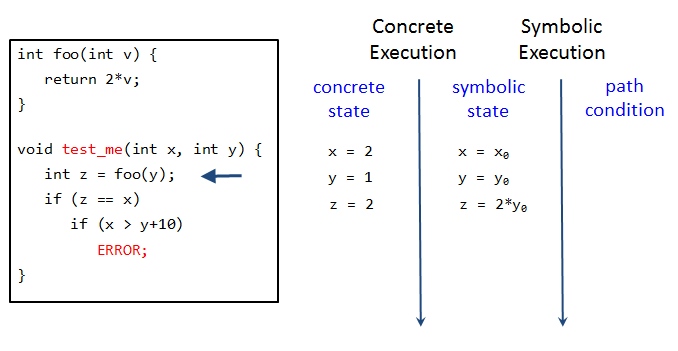
\includegraphics[scale=.4]{dse22.png}
		\end{center}
		\caption{Thực hiện dòng đầu tiên $int z = foo(y)$}
		\label{dse22}
	\end{figure}
\end{center}

Ở dòng kế tiếp, chúng ta kiểm tra tình trạng nhánh $z == x$. Trong trường hợp này, điều kiện là đúng vì vậy điều kiện đường dẫn của chúng ta trở thành $2*y_{0} == x_{0}$. Sau đó DSE kiểm tra dòng tiếp theo của nhánh $true$.

\begin{center}
	\begin{figure}[H]
		\begin{center}
			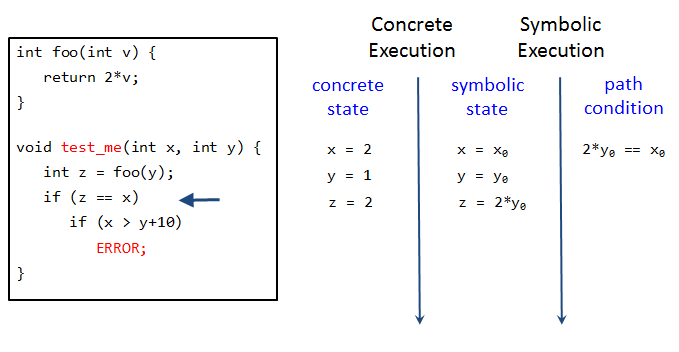
\includegraphics[scale=.4]{dse23.png}
		\end{center}
		\caption{DSE thực hiện điều kiện đường dẫn $true$}
		\label{dse23}
	\end{figure}
\end{center} 

Tại điểm nhánh tiếp theo, $x$ có giá trị cụ thể là $2$ và $y + 10$ có giá trị cụ thể là $11$, vì vậy DSE lấy nhánh $false$, kết thúc chương trình. Thêm ràng buộc tượng trưng $x_{0} <= y_{0} + 10$ vào điều kiện đường dẫn, đây là sự phủ định của điều kiện nhánh mà DSE phát hiện là $fasle$.

\begin{center}
	\begin{figure}[H]
		\begin{center}
			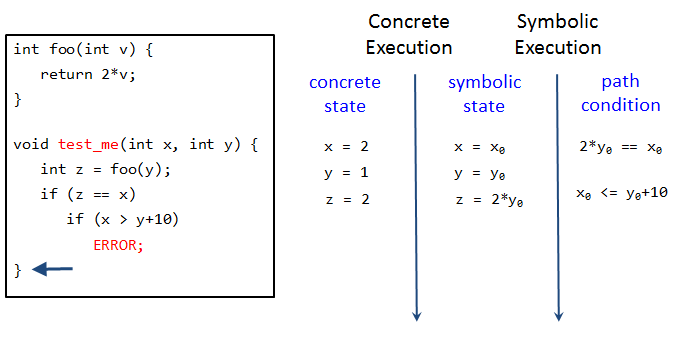
\includegraphics[scale=.4]{dse24.png}
		\end{center}
		\caption{DSE lấy nhánh $false$ kết thúc chương trình}
		\label{dse24}
	\end{figure}
\end{center} 

Vì DSE đã đến cuối chương trình, nó phủ nhận ràng buộc vừa được thêm gần nhất trong điều kiện đường dẫn để có được $ x_{0} > y_{0} + 10 $, và sau đó nó vượt qua các ràng buộc $ 2*y_{0} == x_{0} $ và $ x_{0} > y_{0} + 10$. Để thỏa những ràng buộc này, DSE trả về $x_{0} = 30$ và $y_{0} = 15$.

\begin{center}
	\begin{figure}[H]
		\begin{center}
			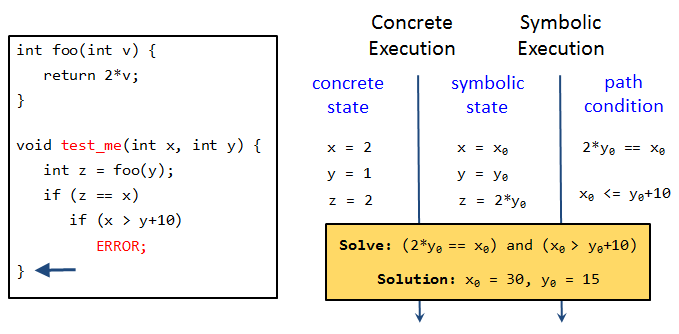
\includegraphics[scale=.4]{dse3.png}
		\end{center}
		\caption{Các giá trị DSE sinh ra sau khi thực thi chương trình lần 2}
		\label{dse3}
	\end{figure}
\end{center}

Bây giờ, DSE chạy hàm test\_me một lần nữa, lần này với các đầu vào $x = 30$ và $y = 15$. Trạng thái biểu tượng các biến bắt đầu $x = x_{0}$ và $y = y_{0}$. $z$ được gán giá trị cụ thể là $30$, trong khi giá trị tượng trưng của nó là $2*y_0$ như những lần chạy trước.

Khi tới điều kiện rẻ nhánh $z == x$, DSE nhận thấy đây là điều kiện $true$, vì vậy DSE thêm điều kiện tượng trưng $2*y_{0} == x_{0}$.

Sau đó tại điểm nhánh tiếp theo, với $x > y + 10$ vì vậy DSE thêm ràng buộc tượng trưng mới $ x_{0} > y_{0}+ 10 $. Nhánh này dẫn đến $ERROR$, tại thời điểm đó chúng ta đã xác định được đầu vào cụ thể làm cho chương trình dẫn đến $ERROR$ là: $x = 30$ và $y = 15$.

\begin{center}
	\begin{figure}[H]
		\begin{center}
			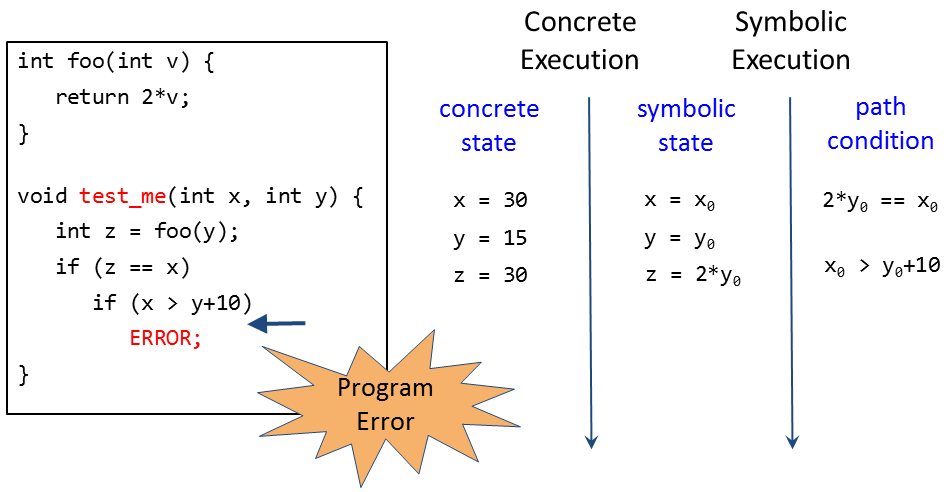
\includegraphics[scale=.4]{dse4.png}
		\end{center}
		\caption{Các giá trị DSE sinh ra sau khi thực thi chương trình lần 3}
		\label{dse4}
	\end{figure}
\end{center}

Kết quả, sau 3 lần chạy chương trình, DSE tạo ra được các cặp giá trị đầu vào có thể duyệt hết các nhánh của chương trình test\_me đó là: $[22,7], [2,1], [30,15]$

\section{Hành vi của chương trình }
Để định lượng hai chương trình tương tự nhau, chúng ta nghiên cứu một số định nghĩa liên quan đến hành vi của hai chương trình như sau:
	
\subsection{Thực thi chương trình}
\begin{definition}\label{def:progexe}
Cho $P$ là một chương trình, $I$ là tập hợp các trị đầu vào của $P$ và $O$ là tập hợp các giá trị đầu ra của $P$. Thực thi chương trình P là ánh xạ $exec: P \times I \rightarrow O$. Với giá trị đầu vào $i \in I$, sau khi thực thi $P$ trên $i$ ta có giá trị đầu ra tương ứng $o \in O$ và ký hiệu $o = exec(P, i)$.  
\end{definition}

\subsection{Độ tương đương về hành vi}
Dựa trên định nghĩa về thực thi chương trình, chúng ta tìm hiểu thế nào là độ tương đương về hành vi giữa hai chương trình thông qua hai chương trình minh họa sau:

{\scriptsize \begin{minipage}[t]{0.45\linewidth}
	\lstinputlisting[label={SwitchCase}, caption = {Switch...Case}]{SwitchCase.cs}
\end{minipage}
\hfill\vrule\hfill
\begin{minipage}[t]{0.45\linewidth}
	\lstinputlisting[label={IfElse}, caption = {If...Else}]{IfElse.cs}
\end{minipage}}


Mã lệnh \ref{SwitchCase} và \ref{IfElse} có tham số đầu vào cùng kiểu giá trị $int$. Mã lệnh \ref{SwitchCase} sử dụng cấu trúc $\textit{\textbf{switch...case}}$, mã lệnh \ref{IfElse} sử dụng cấu trúc $\textit{\textbf{if...else}}$ để kiểm tra giá trị đầu vào $x$. Mặc dù cú pháp sử dụng trong hai chương trình là khác nhau nhưng cách thức xử lý trả về kết quả $y$ là như nhau. Từ đó, chúng ta có thể định nghĩa thế nào là độ tương đương hành vi giữa hai chương trình như sau:

\begin{definition}[Độ tương đương về hành vi]
 Cho $P_{1}$ và $P_{2}$ là hai chương trình có cùng miền các giá trị đầu vào $I$. Hai chương trình này được gọi là tương đương khi và chỉ khi thực thi của chúng giống nhau trên mọi giá trị đầu vào trên $I$, ký hiệu là exec($P_{1}, I$) = exec($P_{2}, I$). 
\end{definition}	

Hai chương trình nếu không tương đương thì sự khác biệt về hành vi, chúng ta tìm hiểu hai mã lệnh sau:

{\scriptsize \begin{minipage}[t]{0.45\linewidth}
	\lstinputlisting[label={KBHV1}, caption = {Chương trình $P_{1}$}]{Khac_biet_HV_1.cs}
\end{minipage}
\hfill\vrule\hfill
\begin{minipage}[t]{0.45\linewidth}
	\lstinputlisting[label={KBHV2}, caption = {Chương trình $P_{2}$}]{Khac_biet_HV_2.cs}
\end{minipage}}


Mã lệnh \ref{KBHV1} và Mã lệnh \ref{KBHV2}  của Chương trình $P_{1}$ và $P_{2}$, cả hai Chương trình có miền giá trị đầu vào cùng kiểu $int$, giá trị trả về của Chương trình $P_{1}$ là $x - 10$, giá trị trả về của Chương tình $P_{2}$ là $x + 10$. Với mọi giá trị của $x$ được thực thi trên cả hai chương trình $P_{1}$ và $P_{2}$ kết quả trả về sẽ không giống nhau. Mặc dù cả hai Chương trình $P_{1}$ và $P_{2}$ có miền giá trị đầu vào như nhau, nhưng hành vi của hai Chương trình hoàn toàn khác nhau. Qua đó, chúng ta có thể định nghĩa sự khác biệt về hành vi như sau:

\begin{definition}[Sự khác biệt hành vi]
Cho $P_{1}$ và $P_{2}$ là hai chương trình có cùng một miền các giá trị đầu vào $I$. Hai chương trình này được xem là có sự khác biêt về hành vi khi và chỉ khi thực thi của chúng khác nhau trên mọi giá trị đầu vào $I$, ký hiệu là $exec(P_{1}, I) \neq exec(P_{2}, I)$.
\end{definition}

\subsection{Độ tương tự hành vi}
Để hiểu thế nào là tương tự hành vi, chúng ta phân tích hai Mã lệnh sau:

{\scriptsize \begin{minipage}[t]{0.45\linewidth}
	\lstinputlisting[label={TTHV1},caption = {Chương trình $P_{1}$}]{TuongTu_HV_1.cs}
\end{minipage}
\hfill\vrule\hfill
\begin{minipage}[t]{0.45\linewidth}
	\lstinputlisting[label={TTHV2}, caption = {Chương trình $P_{2}$}]{TuongTu_HV_2.cs}
\end{minipage}}

Với Mã lệnh \ref{TTHV1} và Mã lệnh \ref{TTHV2} của hai Chương trình $P_{1}$ và $P_{2}$, chúng ta thấy cả hai Chương trình có giá trị đầu vào cùng kiểu dữ liệu là $int$, nếu giá trị đầu vào của biến $x$ nằm trong khoảng $0$ đến $100$ thì giá trị trả về của cả hai Chương trình đều bằng nhau là $x+10$. Ngươc lại, giá trị đầu vào của biến $x$ nằm ngoài khoảng $0$ đến $100$, thì giá trị trả về của Chương trình $P_{1}$ là $x$ và giá trị trả về của Chương trình $P_{2}$ là $-1$. Hai Chương trình $P_{1}$ và $P_{2}$ tuy có kiểu dữ liệu đầu vào như nhau nhưng kết quả đầu ra có thể giống nhau hoặc khác nhau tùy theo giá trị đầu vào của biến $x$. Dựa trên kết quả phân tích, chúng ta định nghĩa độ tương tự hành vi của Chương trình như sau:

\begin{definition}[Độ tương tự hành vi]
Cho $P_{1}$ và $P_{2}$ là hai chương trình có cùng miền giá trị đầu vào $I$, và $I_{s}$ là tập con của $I$. Hai Chương trình được xem là tương tự hành vi khi thực thi chúng giống nhau trên mọi giá trị đầu vào $I_{s}$, ký hiệu  $exec(P_{1}, I_{s}) = exec(P_{2}, I_{s})$ và khác nhau $\forall j \in I \setminus I_{s}$, ký hiệu $exec(P_{1}, j) \neq exec(P_{2}, j)$
\end{definition}

\section{Một số phép đo độ tương tự hành vi}
Để đo độ tương tự về hành vi giữa hai chương trình, chúng ta có thể chạy từng giá trị đầu vào trong miền giá trị đầu vào của hai chương trình. Tỷ lệ giữa số lượng đầu vào thử nghiệm khi thực thi trên cả hai chương trình cho kết quả đầu ra giống nhau trên tổng số lượng đầu vào được thử nghiệm là độ tương tự hành vi giữa hai chương trình. Dựa trên cách tính tỷ lệ kết quả đầu ra của hai chương trình, chúng ta có một số phép đo độ tương tự hành vi như sau:

\subsection{Phép đo lấy mẫu ngẫu nhiên (RS)}
Kỹ thuật của phép đo \textbf{RS} là thực hiện lấy mẫu ngẫu nhiên giá trị đầu vào trên miền giá trị đầu vào của hai chương trình. Thực thi cả hai chương trình trên từng giá trị đầu vào, tiến hành so sánh giá trị kết quả đầu ra của cả hai chương trình. Tỷ lệ giữa tổng số mẫu đầu vào khi thực thi những mẫu này hai chương trình cho kết quả đầu ra có giá trị giống nhau, trên tổng số mẫu đầu vào được thử nghiệm là kết quả cho phép đo RS. Từ đó, chúng ta có định nghĩa phép đo \textbf{RS} như sau:

\begin{definition}[Phép đo RS]
	Cho $P_{1}$ và $P_{2}$ là hai chương trình có cùng miền giá trị đầu vào $I$, $I_{s}$ là tập con ngẫu nhiên của $I$, $I_{a}$ là tập con $I_{s}$. Hai chương trình thực thi giống nhau với $\forall i \in I_{a}$, ký hiệu $exec(P_{1}, i) = exec(P_{2}, i)$ và hai chương trình thực thi khác nhau với $\forall j \in I_{s} \setminus I_{a}$, ký hiệu $exec(P_{1}, j) \neq exec(P_{2}, j)$. Chỉ số phép đo \textbf{RS} được định nghĩa là $M_{RS}(P_{1}, P_{2}) = \left|I_{a}\right| \diagup \left|I_{s}\right| $.
\end{definition}

\begin{algorithm}[H]
	\caption{Phép đo RS}
	\begin{algorithmic}	
		\item $P_{1}, P_{2}:$ Là hai chương trình cần đo độ tương tự
		\item $I$: Miền giá trị đầu vào của $P_{1}, P_{2}$
		\item Set $I_{s} = Random(I)$ \Comment{$I_{s}$: Tập con ngẫu nhiên của $I$}
		\item Set $I_{a} = \emptyset$ 
		\While {$i \in I_{s}$ }  \Comment {Vòng lặp dừng lại khi $\forall i \in I_{s}$ đã được thực thi}
				
				\If{ ($exec(P_{1}, i) = exec(P_{2}, i)$) }
				\State $I_{a} = I_{a} \cup i$		
				\EndIf
		\EndWhile
		\item $M_{RS}(P_{1}, P_{2}) = \left|I_{a}\right| \diagup \left|I_{s}\right| $. 
	\end{algorithmic}
\end{algorithm}


Phép đo \textbf{RS} là một một phép đo đơn giản và hiệu quả để tính độ tương tự của hành vi. Khi miền giá trị của tham số đầu vào rất lớn hoặc vô hạn, phép đo \textbf{RS} thực hiện lấy mẫu ngẫu nhiên để tính toán độ tương tự của hành vi, kết quả đầu ra tương đối tốt và hợp lý so với hành vi thực tế của chương trình. Phép đo \textbf{RS} xử lý, tính toán độ tương tự hành vi dưới dạng hộp đen và không phân tích chương trình để tạo thử nghiệm, nên tốc độ xử lý nhanh và chiếm ít tài nguyên. Mặc khác, phép đo \textbf{RS} không phân tích chương trình để tạo đầu vào thử nghiệm nên phép đo \textbf{RS} có thể bỏ qua một vài tham số đầu vào thử nghiệm có thể được sử dụng để thực thi một số nhánh khác nhau giữa hai chương trình. Vì vậy, phép đo \textbf{RS} không phân biệt được các chương trình có một số hành vi khác nhau. Chúng ta phân tích Mã lệnh $3.7$ và $3.8$ sau để thấy được hạn chế của phép đo \textbf{RS}:

{\scriptsize \begin{minipage}[t]{0.45\linewidth}
	\lstinputlisting[label={RS1}, caption = {Chương trình $P_{1}$}]{RS1.cs}
\end{minipage}
\hfill\vrule\hfill
\begin{minipage}[t]{0.45\linewidth} 
	\lstinputlisting[label={RS2}, caption = {Chương trình $P_{2}$}]{RS2.cs}
\end{minipage}}
 
Chúng ta thấy đoạn Mã lệnh \ref{RS1} và \ref{RS2} của hai Chương trình $P_{1}$ và $P_{2}$ có cùng miền giá trị đầu vào là $string x$, cấu trúc mã lệnh hai chương trình gần như nhau. Nhưng Chương trình $P_{1}$ khác với Chương trình $P_{2}$ đó là sẽ trả kết quả về $0$ nếu tham số đầu vào có giá trị là $XYZ$. Tỷ lệ phép đo \textbf{RS} lấy ngẫu nhiên giá trị đầu vào $x$ trên miền giá trị đầu vào của hai chương trình có giá trị bằng $XYZ$ là rất thấp, vì vậy khả năng câu lệnh $if (x == "XYZ") return 0;$ của Chương trình $P_{1}$ có thể sẽ không được thực thi nên kết quả của phép đo \textbf{RS} sẽ ở mức tương đối so với hành vi thực tế của chương trình.

\subsection{Phép đo tượng trưng trên một chương trình (SSE)}
Phép đo \textbf{SSE} là một phép đo dựa trên số lượng các nhánh đường đi của Chương trình mẫu, mỗi nhánh đường đi của Chương trình mẫu được xem là một hành vi của chương trình. Nếu chọn một giá trị đầu vào thử nghiệm cho một nhánh đường đi trong Chương trình thì các giá trị đầu vào thử nghiệm này sẽ khám phá hết các hành vi trong Chương trình mẫu. Do vậy, số phần tử trong tập các giá trị đầu vào thử nghiệm của phép đo \textbf{SSE} sẽ nhỏ hơn tập các giá trị đầu vào thử nghiệm được chọn theo phương pháp lấy ngẫu nhiên giá trị đầu vào. 

Để tính độ tương tự hành vi của hai chương trình với phép đo \textbf{SSE}, chúng ta chọn Chương trình mẫu làm Chương trình tham chiếu và áp dụng kỹ thuật \textbf{DSE} để tạo ra các đầu vào thử nghiệm dựa trên Chương trình tham chiếu. Sau đó thực thi cả hai chương trình dựa trên các giá trị đầu vào thử nghiệm. Tỷ lệ số lượng các kết quả đầu ra giống nhau của cả hai chương trình trên tổng số các giá trị đầu vào thử nghiệm của Chương trình tham chiếu là kết quả của phép đo \textbf{SSE}. Qua đó, chúng ta có định nghĩa phép đo \textbf{SSE} như sau:

\begin{definition}
	Cho $P_{1}$ và $P_{2}$ là hai chương trình có cùng miền giá trị đầu vào $I$, Chương trình $P_{1}$ là Chương trình tham chiếu, $I_{s}$ là tập các giá trị đầu vào được tạo bởi DSE trên chương trình $P_{1}$, và $I_{a}$ là tập con $I_{s}$. Hai Chương trình thực thi giống nhau với $\forall i \in I_{a}$, ký hiệu $exec(P_{1}, i) = exec(P_{2}, i)$ và hai Chương trình thực thi khác nhau với $\forall j \in I_{s} \setminus I_{a}$, ký hiệu $exec(P_{1}, j) \neq exec(P_{2}, j)$. Chỉ số phép đo \textbf{SSE} được định nghĩa là $M_{SSE}(P_{1}, P_{2}) = \left|I_{a}\right| \diagup \left|I_{s}\right| $.
\end{definition}

\begin{algorithm}[H]
	\caption{Phép đo SSE}
	\begin{algorithmic}	
		\item $P_{1}, P_{2}:$ Là hai chương trình cần đo tương tự
		\item $I$: Miền giá trị đầu vào của $P_{1}, P_{2}$
		\item $P_{1}$: Là Chương trình tham chiếu
		\item Set $I_{s} = DSE(P_{1})$ \Comment{$I_{s}$: Tập đầu vào của $P_{1}$ theo DSE}
		\item Set $I_{a} = \emptyset$ 
		\While{ ($i \in I_{s}$) }  \Comment {Vòng lặp dừng lại khi $\forall i \in I_{s}$ đã được thực thi}
		
		\If{ ($exec(P_{1}, i) = exec(P_{2}, i)$) }
		\State $I_{a} = I_{a} \cup i$		
		\EndIf
		\EndWhile
		\item $M_{SSE}(P_{1}, P_{2}) = \left|I_{a}\right| \diagup \left|I_{s}\right| $. 
	\end{algorithmic}
\end{algorithm}

Ngược lại với phép đo RS, phép đo SSE khám phá những đường đi khả thi khác nhau trong chương chình tham chiếu để tạo dữ liệu đầu vào của chương trình. Do đó, các đầu vào thử nghiệm này sẽ thực thi hết các đường đi của chương trình tham chiếu và có khả năng phát hiện được những chương trình cần tính có những hành vi khác so với Chương trình tham chiếu. Những phép đo SSE vẫn còn hạn chế, đó là phép đo SSE không xem xét đường đi của Chương trình cần phân tích để tạo các giá trị đầu vào thử nghiệm mà chỉ dựa vào các đầu vào thử nghiệm được phân tích từ Chương trình tham chiếu. Các đầu vào thử nghiệm này không nắm bắt được hết các hành vi của Chương trình cần phân tích, Chương trình cần phân tích có thể sẽ có những hành vi khác so với Chương trình tham chiếu. Một số chương trình có thể có những vòng lập vô hạn phụ thuộc vào giá trị đầu vào nên SSE không thể liệt kê được tất cả các đường dẫn của chương trình. Chúng ta xem xét và phân tích 2 đoạn Mã lệnh $3.9$ và $3.10$ để thấy được hạn chế của phép đo SSE như sau:

{\scriptsize \begin{minipage}[t]{0.45\linewidth}
	\lstinputlisting[label={SSE1}, caption = {Chương trình $P_{1}$}]{SSE1.cs}
\end{minipage}
\hfill\vrule\hfill
\begin{minipage}[t]{0.45\linewidth}
	\lstinputlisting[label={SSE2}, caption = {Chương trình $P_{2}$}]{SSE2.cs}
\end{minipage}}

Hai đoạn Mã lệnh \ref{SSE1} và Mã lệnh \ref{SSE2} của hai Chương trình $P_{1}$ và $P_{2}$, chọn Chương trình $P_{1}$ làm Chương trình tham chiếu, sử dụng kỹ thuật \textbf{DSE} để phân tích chương trình $P_{1}$ ta được tập các giá trị đầu vào thử nghiệm là ${(0, 1)}$. Trong khi đó, phân tích Chương trình $P_{2}$ chúng ta được tập các giá trị đầu vào thử nghiệm của Chương trình $P_{2}$  là ${(0, 1, 2)}$. Do đó, chúng ta thấy tập giá trị đầu vào thử nghiệm do phép đo \textbf{SSE} tạo ra thiếu giá trị đầu thử nghiệm $2$ để có thể thực thi hết các đường đi của Chương trình $P_{2}$.

\subsection{Kỹ thuật thực thi chương trình kết hợp (PSE)}
Để giải quyết giới hạn của phép đo \textbf{SSE} khi tạo ra tập các giá trị đầu vào thử nghiệm không thực thi hết các các đi của Chương trình cần phân tích. Phép đo \textbf{PSE} giải quyết giới hạn của phép đo \textbf{SSE} bằng cách tạo một Chương trình kết hợp giữa Chương trình cần phân tích với Chương trình tham chiếu. Dựa trên Chương trình kết hợp sử dụng kỹ thuật \textbf{DSE} để tạo ra đầu vào thử nghiệm cho cả hai chương trình, các đầu vào thử nghiệm này bao gồm các đầu vào thử nghiệm đúng và không đúng. Các đầu vào thử nghiệm đúng là những giá trị khi thực thi trên cả hai chương trình sẽ cho kết quả đầu ra như nhau, ngược lại các đầu vào thử nghiệm không đúng là những giá trị khi thực thi trên cả hai chương trình sẽ cho kết quả khác nhau. Do đó, phép đo \textbf{PSE} được tính bằng tỷ lệ các giá trị đầu vào thử nghiệm đúng trên tổng số các giá trị đầu vào được thử nghiệm. 

\newpage
\lstinputlisting[label={PSE}, caption = {Chương trình kết hợp PSE}]{PSE.cs}

Dựa trên cách thức hoạt động của phép đo \textbf{PSE}, chúng ta có định nghĩa phép đo \textbf{PSE} như sau:
\begin{definition}[Phép đo PSE]
	Cho $P_{1}$ và $P_{2}$ là hai Chương trình có cùng miền giá trị đầu vào $I$. $P_{3}$ là Chương trình
	kết hợp của $P_{1}$ và $P_{2}$, ký hiệu $(exec(P_{1}, I) =  exec(P_{2}, I))$.  $I_{s}$ là tập các giá trị đầu vào được tạo bởi \textbf{DSE} từ Chương trình $P_{3}$, $I_{a}$ là tập con $I_{s}$. Hai Chương trình $P_{1}$ và $P_{2}$ thực thi giống nhau khi Chương trình $P_{3}$ thực thi cho giá trị đúng với $\forall i \in I_{a}$, ký hiệu $exec(P_{3}, i) = T$, và $\nexists j \in I_{s} \backslash I_{a}$ thực thi Chương trình $P_{3}$ cho giá trị đúng. Chỉ số phép đo \textbf{PSE} được định nghĩa là $M_{PSE}(P_{1}, P_{2}) = \left|I_{a}\right| \diagup \left|I_{s}\right| $.
\end{definition}

\begin{algorithm}[h]
	\caption{Phép đo PSE}
	\begin{algorithmic}	
		\item $P_{1}, P_{2}$: Là hai chương trình cần đo tương tự
		\item $I$: Miền giá trị đầu vào của $P_{1}, P_{2}$
		\item $P_{3}$: Là Chương trình kết hợp của $P_{1}, P_{2}$, ký hiệu  $(exec(P_{1}, I) = exec(P_{2}, I))$
		\item Set $I_{s} = DSE(P_{3})$ \Comment{$I_{s}$: Tập đầu vào của $P_{3}$ theo DSE}
		\item Set $I_{a} = \emptyset$ 
		\While{$i \in I_{s}$} \Comment {Vòng lặp dừng lại khi $\forall i \in I_{s}$ đã được thực thi} 		
			\If{ ($exec(P_{1}, i) = exec(P_{2}, i)$) }
			\State $I_{a} = I_{a} \cup i$		
			\EndIf
		\EndWhile
		\item $M_{PSE}(P_{1}, P_{2}) = \left|I_{a}\right| \diagup \left|I_{s}\right| $. 
	\end{algorithmic}
\end{algorithm}

Phép đo \textbf{PSE} đã cải thiện được hạn chế của phép đo \textbf{SSE} khi dữ liệu thử nghiệm được  tạo ra từ trên Chương trình kết hợp, tập dữ liệu thử nghiệm có khả năng thực thi hết các nhánh đường đi của Chương trình tham chiếu và Chương trình cần tính. Tuy nhiên, phép đo \textbf{PSE} cũng có hạn chế trong quá trình xử lý các vòng lặp lớn hoặc vô hạn. Để giảm bớt hạn chế này, chúng ta có thể giới hạn miền đầu vào hoặc đếm số vòng lặp của các Chương trình. Ngoài ra, phép đo \textbf{PSE} khám phá đường dẫn của Chương trình kết hợp nên quá trình xử lý sẽ tốn thời gian và tài nguyên hơn so với phép đo \textbf{SSE} khi chỉ khám phá đường dẫn của Chương trình tham chiếu.
  